\documentclass[a4paper,titlepage]{article}
\usepackage[utf8]{inputenc} %Make sure all UTF8 characters work in the document
\usepackage{listings} %Add code sections
\usepackage{color}
\usepackage{graphicx}
\usepackage{titling}
\usepackage{textcomp}
\usepackage[hyphens]{url}
\usepackage[bottom]{footmisc}
\usepackage[yyyymmdd]{datetime}
\definecolor{listinggray}{gray}{0.9}
\definecolor{lbcolor}{rgb}{0.9,0.9,0.9}

%Set page size
\usepackage{geometry}
\geometry{margin=3cm}
\usepackage{parskip} 

\renewcommand{\dateseparator}{-}

\title{
\textbf{Kravspecifikation - The Gentoo Saga} \\
\subtitle{TSEA83 Grupp 33}
\author{
    Emil Segerbäck - emise935\\Malcolm Vigren - malvi108\\Robin Sliwa - robsl733
  }
  \\
\date{\today}
}

\begin{document}
	\maketitle
	\newpage

\section{Inledning}
Vi ska göra en dator som ska kunna köra ett enkelt plattformspel, 
i stil med t.ex. Super Mario. Spelaren styr en åsnepingvin med ett USB-tangentbord,
ljudeffekter/spelmusik ska spelas i fyrkantsvågor genom den enkla 
monohögtalaren och själva spelet ska visas på en VGA-skärm.

Vi tänker oss att CPU:n ska ha en pipelinead arkitektur.

\section{Grovt blockschema}
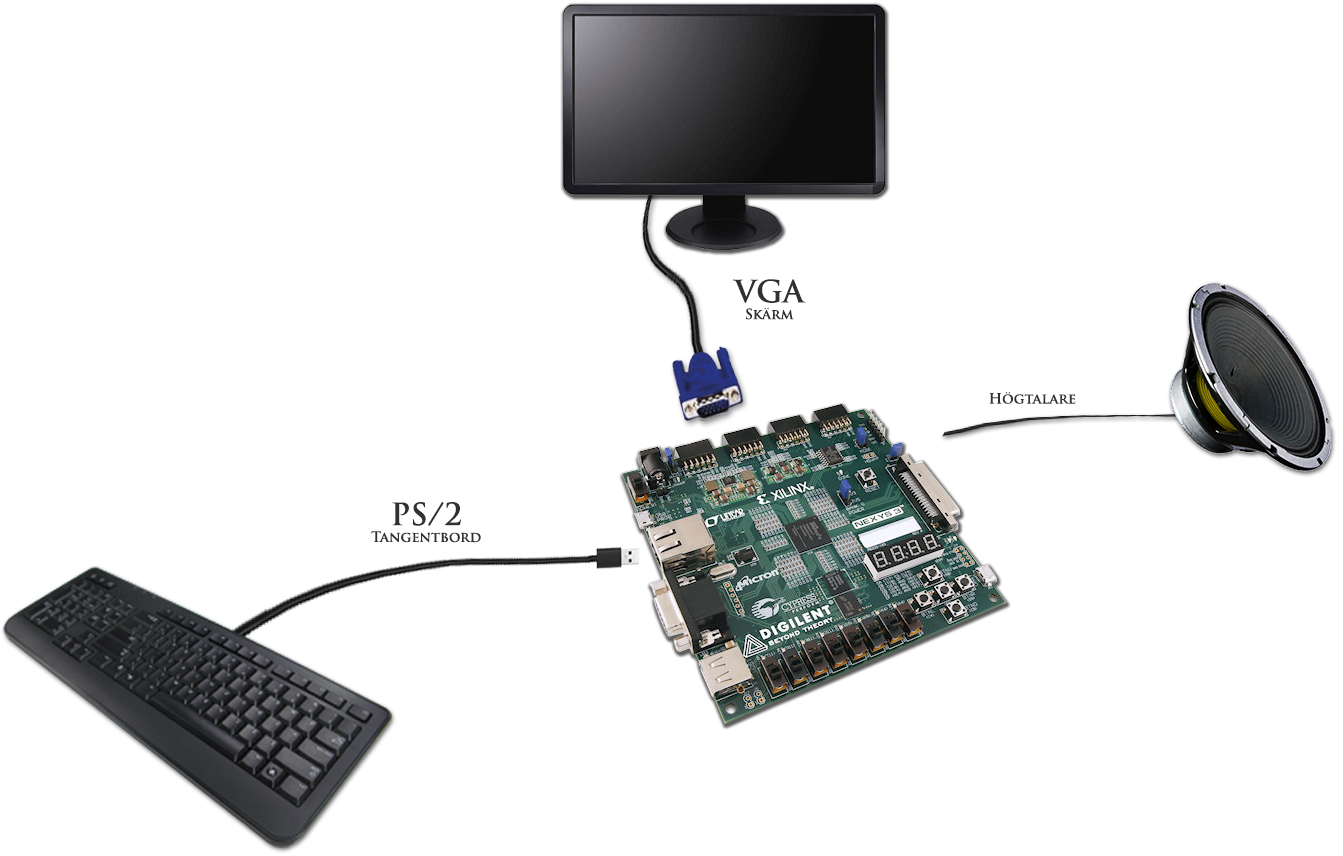
\includegraphics[width=14cm]{blockschema.png}

\section{Kravslista}
Vår dator \textbf{ska} ha:
\begin{itemize}
    \item VGA-skärm med en upplösning på 640x480 pixlar med 8bitars grafik
    \item Skärmuppdelning bestående av tiles som ska vara 16x16 pixlar
    \item Sprites som visas på skärmen med samma storlek som en tile
	\item Tangentbordsstyrning
    \item Musik
    \item En accelererad gravitation (mer realistisk)
\end{itemize}
Vår dator \textbf{bör} ha:
\begin{itemize}
	\item Möjlighet för inladdning av banor
	\item Passande ljudeffekter 
	\item Flera typer av fiender
\end{itemize}
\end{document}
